\section{A case study: \texorpdfstring{$D_4$}{D4}}
\label{sec:a_case_study__d4}

\newcommand{\InvVector}[5]{\psi (
    j_{#1} m_{#1}
    j_{#2} m_{#2}
    j_{#3} n_{#3}
    j_{#4} n_{#4}
    | a_{#5}
)}
\newcommand{\InvVectorPrime}[5]{\psi (
    j_{#1}^\prime m_{#1}^\prime
    j_{#2}^\prime m_{#2}^\prime
    j_{#3}^\prime n_{#3}^\prime
    j_{#4}^\prime n_{#4}^\prime
    | a_{#5}^\prime
)}


In this section we consider pure gauge theory with gauge group $G=D_4$, the dihedral group with eight elements, on a small $2 \times 2 $ periodic lattice (see Fig.~\ref{fig:periodic plaquette}).
We compute the Hamiltonian in the gauge-invariant spin-network basis and diagonalize it exactly.

\subsection{Implementation of the physical Hilbert space}
\label{sub:implementation_of_the_physical_hilbert_space}

As remarked in Sec.~\ref{sub:dimension_physical_hilbert_space}, the physical Hilbert space of this theory has dimension equal to $8960$ and it's not practical to store the gauge-invariant states directly.
Instead, we compute numerically the basis of invariant states at a site for all possible combinations of irreps assigned to the four links attached to the site.
In other words, we compute the coefficients $\psi$ of \eqref{eq:invariant states at a site}.

Then, the gauge-invariant states can be stored just as labels of the choice of \acp{irrep} on the links, and invariant vectors at each site.
When the coefficients of a physical state are needed, it is sufficient to call the appropriate $\psi$'s based on the label of the state.
Therefore one has to store just the invariant vectors of a single vertex and the labels of the physical states, without needing to expand \eqref{eq:spin network states 2x2} and save the full result.
This greatly cuts down on the amount of memory necessary for storing the gauge-invariant basis.

Let's try to quantify this gain.
In the $D_4$ gauge theory in two dimensions, we found that the total number of invariant vectors for a vertex is $164$.
The size of the invariant vectors depends on the \acp{irrep} configuration around the vertex, but they are at most $16$-dimensional.
Using single-precision float (which requires $4 \mathrm{B}$), in the worst case scenario (all vectors are $16$-dimensional) the storage for the invariant vectors would require only around $10 \mathrm{KB}$.
This is a fixed storage cost independent of the lattice size.
On a $2 \times 2$ periodic lattice, in order to label the states we would need $8$ integers (\ac{irrep} index) plus $4$ integers (invariant vector choice at each vertex).
With $8960$ states and $2 \mathrm{B}$ per integer, the total storage cost would amount to $\sim \! 230 \mathrm{KB}$, a huge decrease from the $600 \mathrm{GB}$ estimated before.
In the case of a $3 \times 3$ lattice, the storage cost would increase to $\sim \! 15 \mathrm{GB}$, orders of magnitude less than $2 \times 10^{16} \mathrm{GB}$.
Using these coefficients $\psi$, we then compute the matrix elements of the electric and magnetic Hamiltonians separately in the spin-network basis \eqref{eq:spin network states 2x2}.


\subsection{Explicit computation of the Hamiltonian}
\label{sub:explicit_computation_of_the_hamiltonian}

The electric Hamiltonian is diagonal, and the magnetic Hamiltonian is off-diagonal.
In units of $\lambda_E + \lambda_B$ the Hamiltonian can be written as
\begin{equation}
    H = \lambda H_E + (1-\lambda) H_B
    \quad \text{where} \quad
    \lambda = \frac{\lambda_E}{\lambda_E + \lambda_B} \in [0, 1].
\end{equation}
In practice, for each $\lambda$, $H$ is a $8960 \times 8960$ matrix.
As expected for spin-network states \cite{burgio2000physical}, we find $H$ to be very sparse: around $1\%$ of the elements are non-zero.
A plot of the non-zero elements elements of $H_B$ is shown in Fig.~\ref{fig:magn_sparse}.

The electric and magnetic Hamiltonians were chosen as in \eqref{eq:generalized ym hamiltonian}.
In particular, we chose $h_B = -2 \tr \rho_4$ where $\rho_4$ is the two-dimensional irrep of $D_4$ and considered the three different choices of the set $\Gamma$ for $h_E$ described in Sec.~\ref{sub:the_finite_group_laplacian}.
These are:
\begin{equation*}
    \begin{split}
        \Gamma_1 & = \{r,r^3,s,r^2s\}, \\
        \Gamma_2 & = \{r, r^3, s, rs, r^2s, r^3s\}, \\
        \Gamma_3 & = \{r, r^2, r^3\}.
    \end{split}
\end{equation*}
We recall that the electric Hamiltonian is two-fold degenerate on each link with $\Gamma_3$ but is not degenerate for $\Gamma_1, \Gamma_2$.
The choice of $\Gamma_2$, unlike the other two, gives rise to a Lorentz-invariant theory.

Working in the spin state basis, computing the matrix elements of $H_E = \sum_{\link} h_E$ is rather easy, because is diagonal in the \ac{irrep} basis:
\begin{equation}
    \mel{ \{j\}^{\prime}, A^{\prime}}{H_E}{ \{j\}, A} =
    \delta( \{j\}, \{j\}^{\prime}) \delta(A, A^{\prime}) \sum_{\link \in \Lattice} f(j_{\link})
\end{equation}
The difficult part comes from the magnetic Hamiltonian $H_B = \sum_{\plaquette} h_B(g_{\plaquette})$.

In order to compute the matrix elements of $H_B$, one can use the group elements base, where it is diagonal.
In this basis we have
\begin{equation}
    \tr \rho_4 =
    2 \sum_{g_1 \cdots g_4} \Re \chi_4(g_{\plaquette}) \ketbra{g_1 g_2 g_3 g_4}{g_1 g_2 g_3 g_4}.
    \label{eq:plaquette_group_basis}
\end{equation}
The above $\ket{g_1 g_2 g_3 g_4}$ can shorten as $\ket{g_{\plaquette}}$.
We denote with $\ket{ \{jmn\}_{\plaquette}}$ the state $\ket{j_1 m_1 n_1 \cdots j_4 m_4 n_4}$ for the links around the plaquette $\plaquette$.
Then, a matrix element of \eqref{eq:plaquette_group_basis} in the $\ket{ {jmn}_{\plaquette}}$ basis can be computed as
\begin{equation}
    \mel{ \{jmn\}_{\plaquette}^{\prime}}{ \tr \rho_4}{ \{jmn\}_{\plaquette}} =
    2 \sum_{g_{\plaquette}} \Re \chi_4 (g_{\plaquette})
        \braket{ \{jmn\}_{\plaquette}^{\prime} }{g_{\plaquette}}
        \braket{g_{\plaquette}}{ \{jmn\}_{\plaquette} }
    \label{eq:plaquette_terms}
\end{equation}
The terms $\braket{ \{jmn\}_{\plaquette} }{ g_{\plaquette} }$ can be obtained from \eqref{eq:change_of_basis}.
The coefficients \eqref{eq:plaquette_terms} depends on the representations and can be precomputed.
We will refer to then as $C( \{jmn\}_{\plaquette}^{\prime}, \{jmn\}_{\plaquette})$.

These coefficients can be used to compute the matrix elements of $H_B$ in the full (non gauge-invariant) \ac{irrep} basis $\ket{ \{jmn\} }$:
\begin{multline}
    \mel{ \{jmn\}^{\prime} }{H_B}{ \{jmn\} } =
    - \sum_{\plaquette}
        \qty(
            \prod_{\link \in \plaquette} \delta( j_{\link}^{\prime} m_{\link}^{\prime} n_{\link}^{\prime}, j_{\link} m_{\link} n_{\link} )
        ) \times \\
        \times C( \{jmn\}_{\plaquette}^{\prime}, \{jmn\}_{\plaquette}).
\end{multline}
Thus, using \eqref{eq:spin network states 2x2}, we finally obtain the expression for the magnetic in the gauge-invariant basis:
\begin{equation}
    \begin{split}
        \mel{ \{j\}^{\prime}, A^{\prime}}{H_B}{ \{j\}, A} & =
        - \sum_{\plaquette} \sum_{ \{mn\} } \sum_{ \{mn\}^{\prime} }
            \qty(
                \prod_{\link \in \plaquette} \delta( j_{\link}^{\prime} m_{\link}^{\prime} n_{\link}^{\prime}, j_{\link} m_{\link} n_{\link} )
            ) \\
            & \times C( \{jmn\}_{\plaquette}^{\prime}, \{jmn\}_{\plaquette}) \\
            & \times \InvVectorPrime{1}{4}{5}{8}{1} \InvVector{1}{4}{5}{8}{1} \\
            & \times \InvVectorPrime{5}{2}{1}{7}{2} \InvVector{5}{2}{1}{7}{2} \\
            & \times \InvVectorPrime{6}{7}{3}{2}{3} \InvVector{6}{7}{3}{2}{3} \\
            & \times \InvVectorPrime{3}{8}{6}{4}{4} \InvVector{3}{8}{6}{4}{4}.
    \end{split}
    \label{eq:explicit_magn_Hamiltonian}
\end{equation}

\begin{figure}[t]
    \centering
    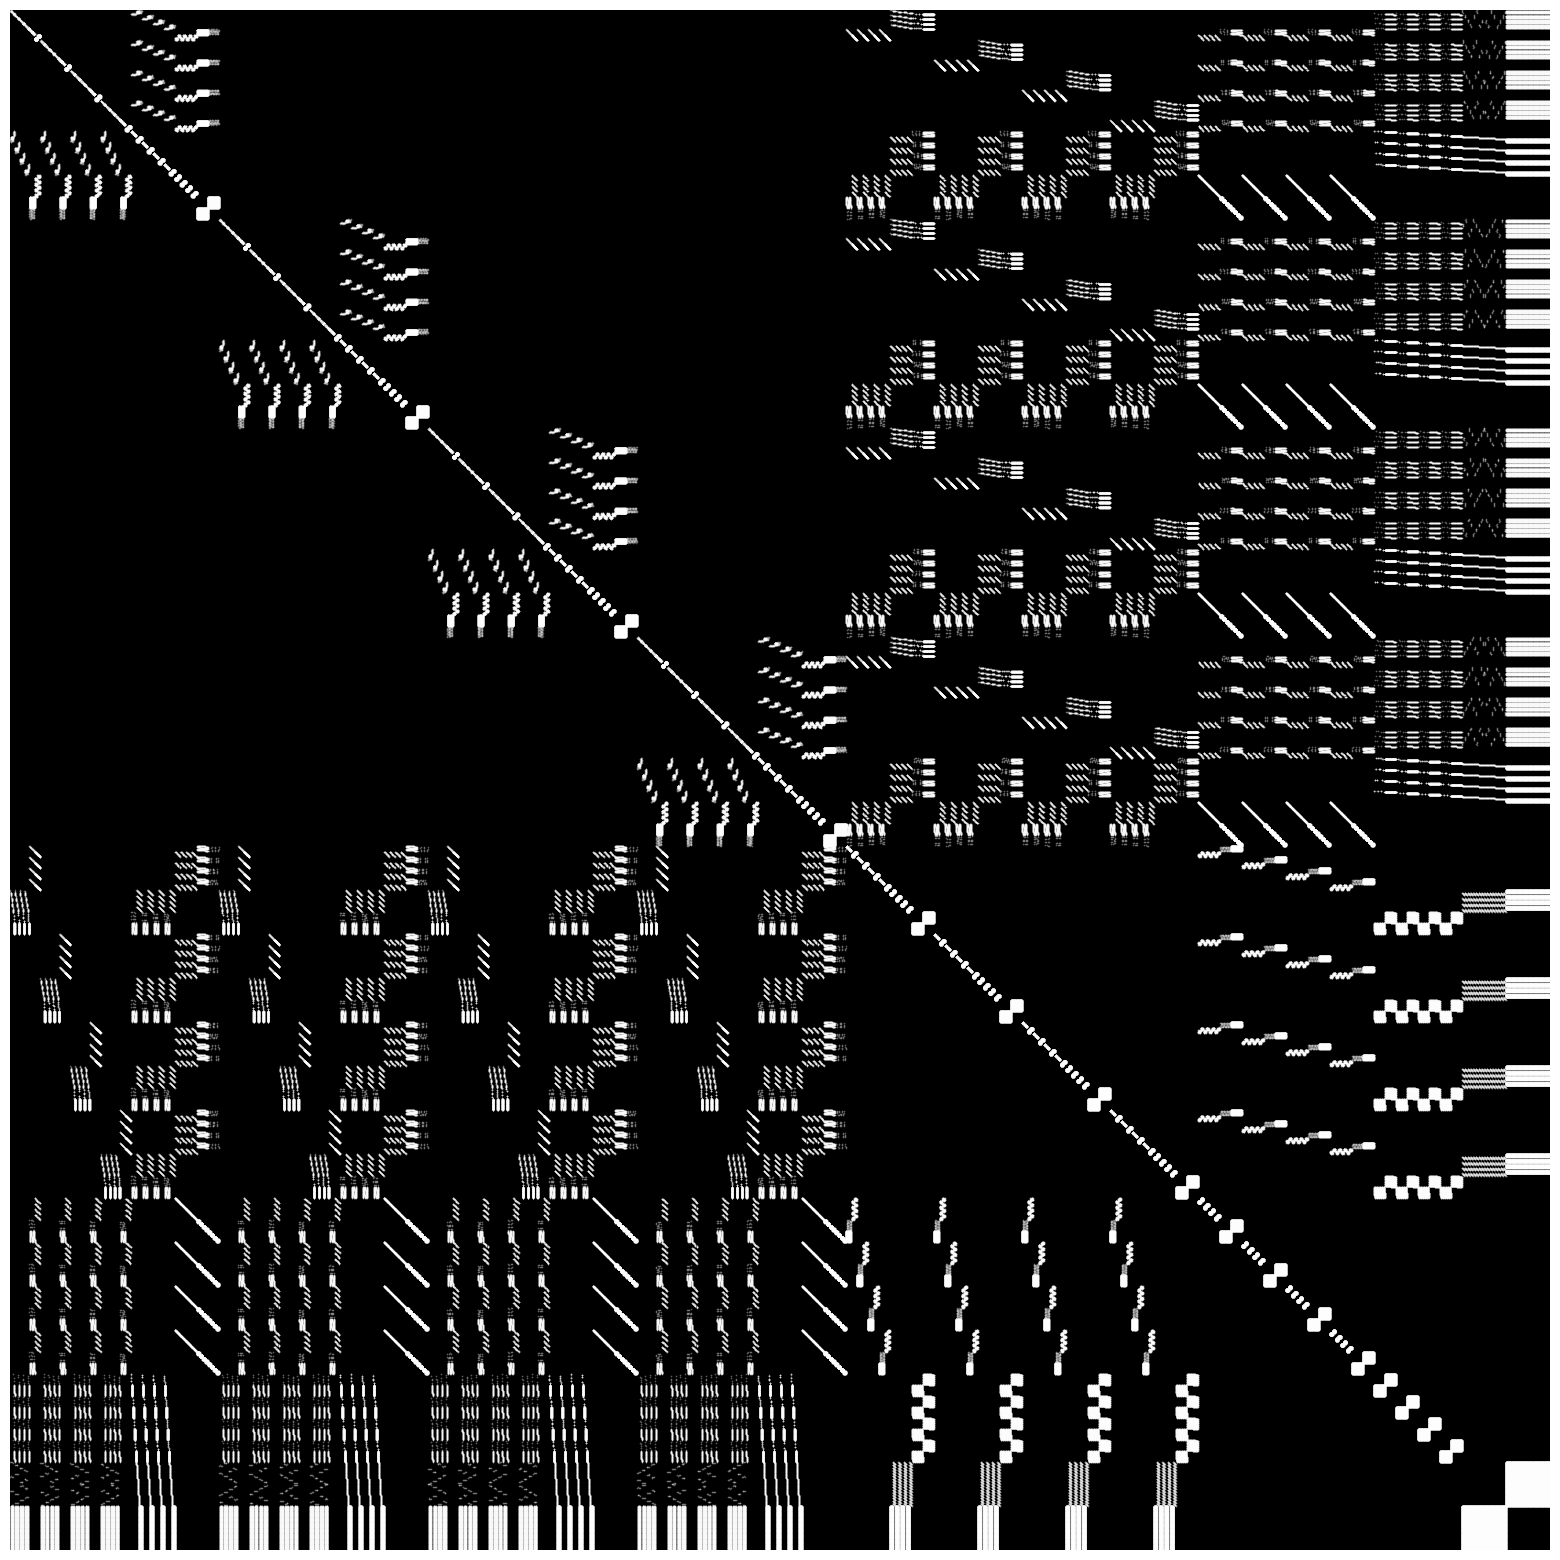
\includegraphics[width=7cm]{assets/graphs/magn_sparse.png}
    \caption[Non-zero elements of $H_B$]{%
        Plot of the $8960$-dimensional Hamiltonian matrix $H_B$.
        % Plot of the elements of the magnetic Hamiltonian $H_B$.
        The non-zero elements are presented as white dots, which have been enlarged in order to make them visible against the black background.
        It can be noticed that there is a lot of regular structure, which suggests that may be methods for further compressing the Hamiltonian.
        Note that the diagonal lines are just slightly offset from the true diagonal at the matrix, which contains only zeros.
    }
    \label{fig:magn_sparse}
\end{figure}


Notice that when $\ket{ \{j\}^{\prime}, A^{\prime}}$ and $\ket{ \{j\}, A}$ are fixed, only the indices $ \{mn\} $ and $ \{mn\}^{\prime}$ are free.
Additionally, each index $m$ or $n$ of the invariant vectors $\psi$ is contracted with an index of the plaquette coefficients $C$.
The same goes for the primed indices.
This means that the terms of the sum over the plaquette can be computed as \emph{tensor contractions}.
Using numerical libraries that efficiently implements tensors, one can greatly improve the computation time.

Another note that is important to point out is the role of the delta functions in \eqref{eq:explicit_magn_Hamiltonian}.
These are what make the magnetic Hamiltonian sparse, combined with the structure of $C$.
The only non-zero matrix elements are only those between two states whose \ac{irrep} configuration coincide outside a plaquette $\plaquette$.
Then, inside the plaquette $\plaquette$ also the coefficients $C$'s has to be non-zero.
It is easy to see that these two facts greatly restrict what matrix elements of $H_B$ can be non-zero.



\subsection{Numerical results}
\label{sub:numerical_results_D4}

\subsubsection*{Ground state energy and gap}

Looking at the ground state energy in Fig.~\ref{fig:ground_state_energy_D4}, one sees that the system evolves from a electric ground state to a magnetic one, with a transition around $0.6 \lesssim \lambda \lesssim 0.8$, for all three case.
This is because the Hamiltonian at $\lambda = 0$ coincide with $H_E$ and $h_E$ has always a zero eigenvalue, while at $\lambda=1$ the Hamiltonian reduces to $H_B$, which is the same in all three cases.
Therefore, a transition is expected for an intermediate value of $\lambda$.

The energy gap corresponds to the difference $E_1 - E_0$, where $E_1$ is the energy of the first excited state.
When the energy gaps are considered, we notice a clear difference between $\Gamma_3$ and the rest.
For $\Gamma_1$ and $\Gamma_2$ the gap closes, signalling the aforementioned transition.
While for $\Gamma_3$ the picture is quite different.
The electric Hamiltonian is degenerate, as it is expected from the fact that $\Gamma_3$ does not generate the whole $D_4$.
This degeneracy is slightly lifted for $\lambda > 0$ but the scale of the gap remains much smaller than in the other two cases.
At this lattice size we are not able to exclude finite size effects for this lifted degeneracy.

\subsubsection*{Electric and magnetic expectation values}

The ground state expectation values of the electric and magnetic Hamiltonians are shown in Fig.~\ref{fig:HE_HB_expt_val_D4}.
The plaquette Wilson loop is equal to $H_B$ apart from an overall prefactor of $8$, and therefore its behaviour is also shown in Fig.~\ref{fig:HE_HB_expt_val_D4} (right).
We note that our data for the ground state energies agrees with that obtained in \cite{marchesethesis} with a different method.

One possible way to locate the transition point is to identify it as the point of sharpest variation of $\expval{H_E}$ and/or $\expval{H_B}$ (i.e. the maximum of the absolute value of their derivative with respect to $\lambda$).
With this identification, the transition points given by either $\expval{H_E}$ or $\expval{H_B}$ coincide at $\lambda_1^* = 0.67(1)$ and $\lambda_2^* = 0.76(1)$ for $\Gamma_1$ and $\Gamma_2$, but show a small difference for $\Gamma_3$, at $\lambda_{3,E}^* = 0.63(1)$ and $\lambda_{3,B}^* = 0.61(1)$.

\subsubsection*{Fidelity susceptibility}

Another way to locate the transition points is through the peaks of \emph{fidelity susceptibility} \cite{you2007fidelity, wang2016fidelity}.
Calling $\ket{\psi_0(\lambda)}$ the ground state of $H(\lambda)$, one can look at the fidelity susceptibility
\cite{you2007fidelity}
\begin{equation}
    \chi(\lambda) = -\frac{\partial^2}{\partial \epsilon^2} \log \abs{\expval{\psi_0(\lambda) | \psi_0(\lambda+\epsilon) }}^2 \bigg\lvert_{\epsilon=0},
\end{equation}
which is expected to peak at the transition \cite{wang2016fidelity}.
Fig.~\ref{fig:fidelity_D4} shows $\chi(\lambda)$ for the three cases and its peak identifies the transition point as $\lambda_{1, \chi}^*=0.67(1)$, $\lambda_{2, \chi}^*=0.76(1)$ and $\lambda_{3, \chi}^*=0.62(1)$, in agreement with the previous method.

\bigbreak

Overall, these results point towards the expected picture of a two-phase structure for all three cases.
The data for $\Gamma_1$ and $\Gamma_2$ is consistent with the usual picture of a confining phase at small $\lambda$ and a deconfined phase at large $\lambda$.
For $\Gamma_3$, the gap is much smaller, especially at small $\lambda$, which complicates the interpretation of this phase as confining.
Of course, due to the small volume these results are only qualitative and preliminary; a study with larger volumes would be required in order to properly establish the phase structure.
However, they point to the possibility that theories with electric degeneracy may display different behaviour and phase structure compared to those with no electric degeneracy.

\newpage

\vspace*{1cm}

\begin{figure}[h]
    \centering
    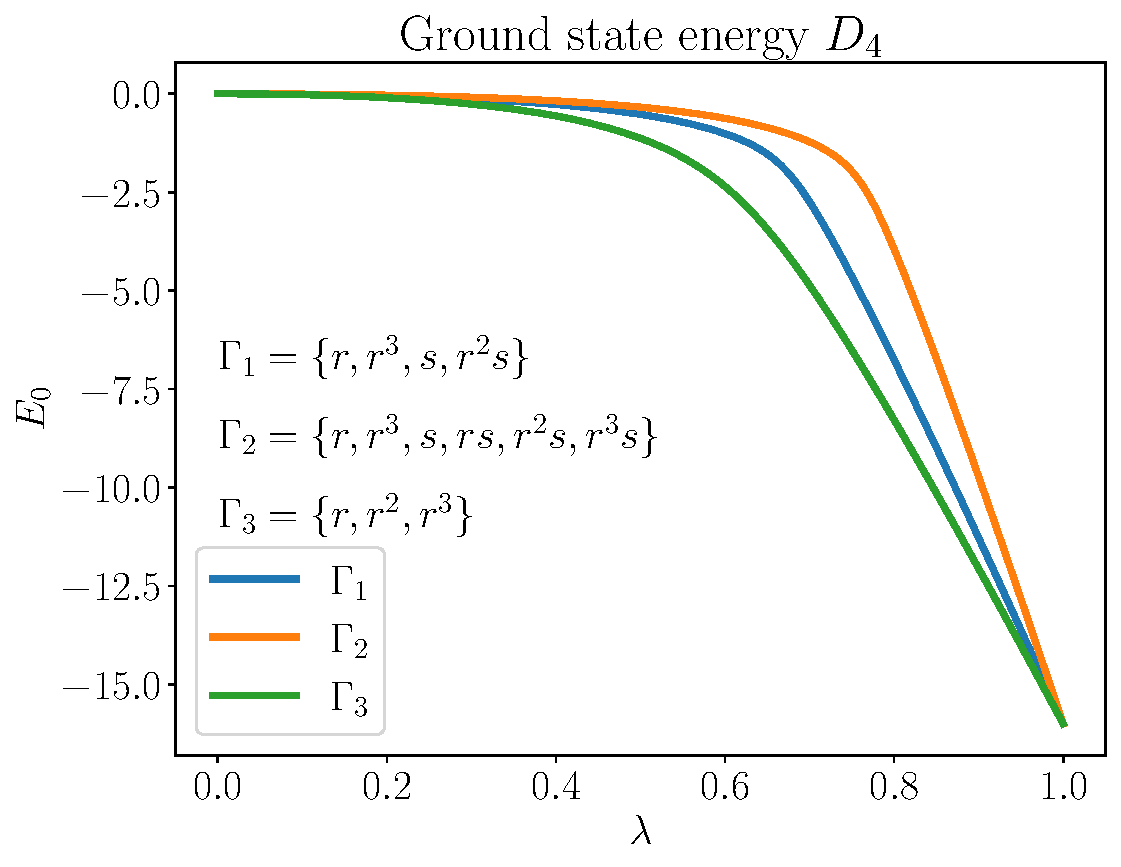
\includegraphics[width=8cm]{assets/graphs/gs_energy_comparison_1_2_3.pdf}
    \caption[Ground state energy for $D_4$]{Ground state energy of the $D_4$ gauge theory, for the three different generating $\Gamma_1$, $\Gamma_2$ and $\Gamma_3$.
        For $\lambda=1$, the Hamiltonian is equivalent for all the three cases, because is just $H_B$.
        While, for $\lambda=0$ the ground state energy is zero because in all thee cases $H_E$ has always zero eigenvalues.
        It can be seen that the transition points is always in the region $ 0.6 \lesssim \lambda \lesssim 0.8$.
    }%
    \label{fig:ground_state_energy_D4}
\end{figure}

\vspace*{0.5cm}

\begin{figure}[h]
    \centering
    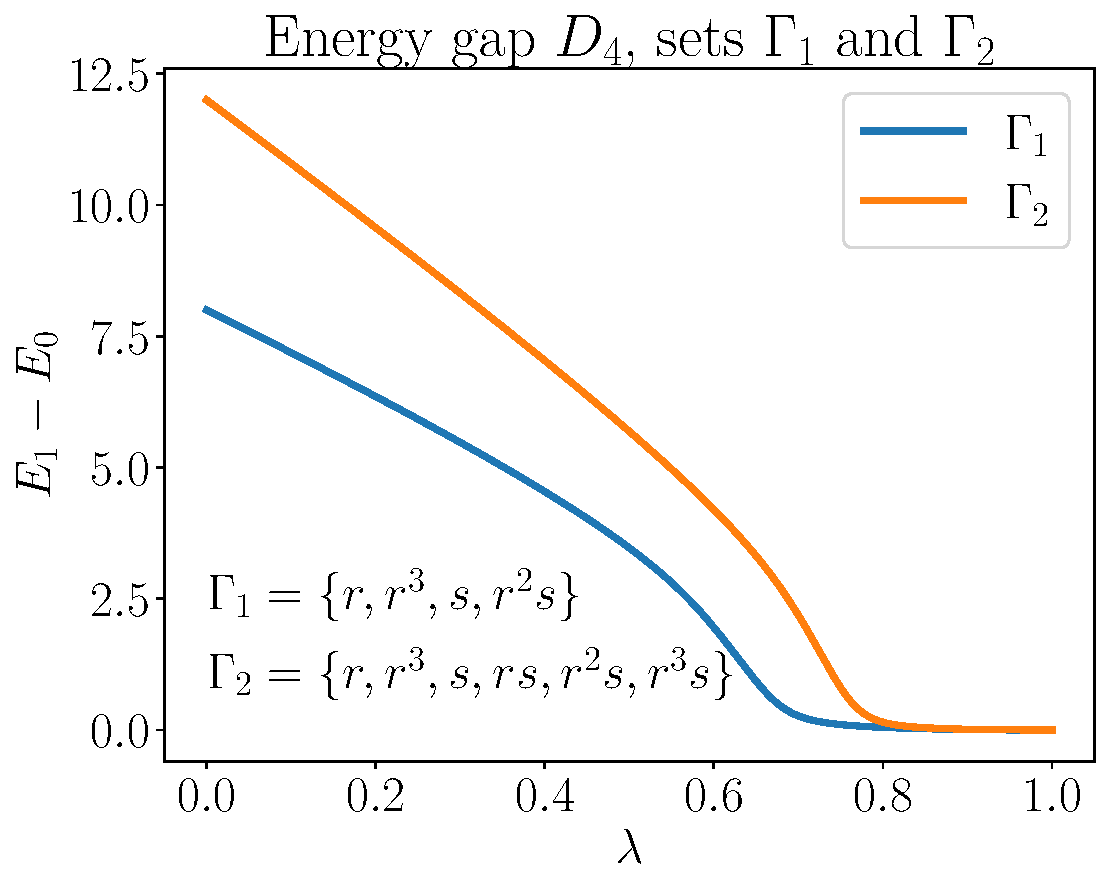
\includegraphics[height=5cm]{assets/graphs/energy_gap_D4_1_2.pdf}
    \hfill%
    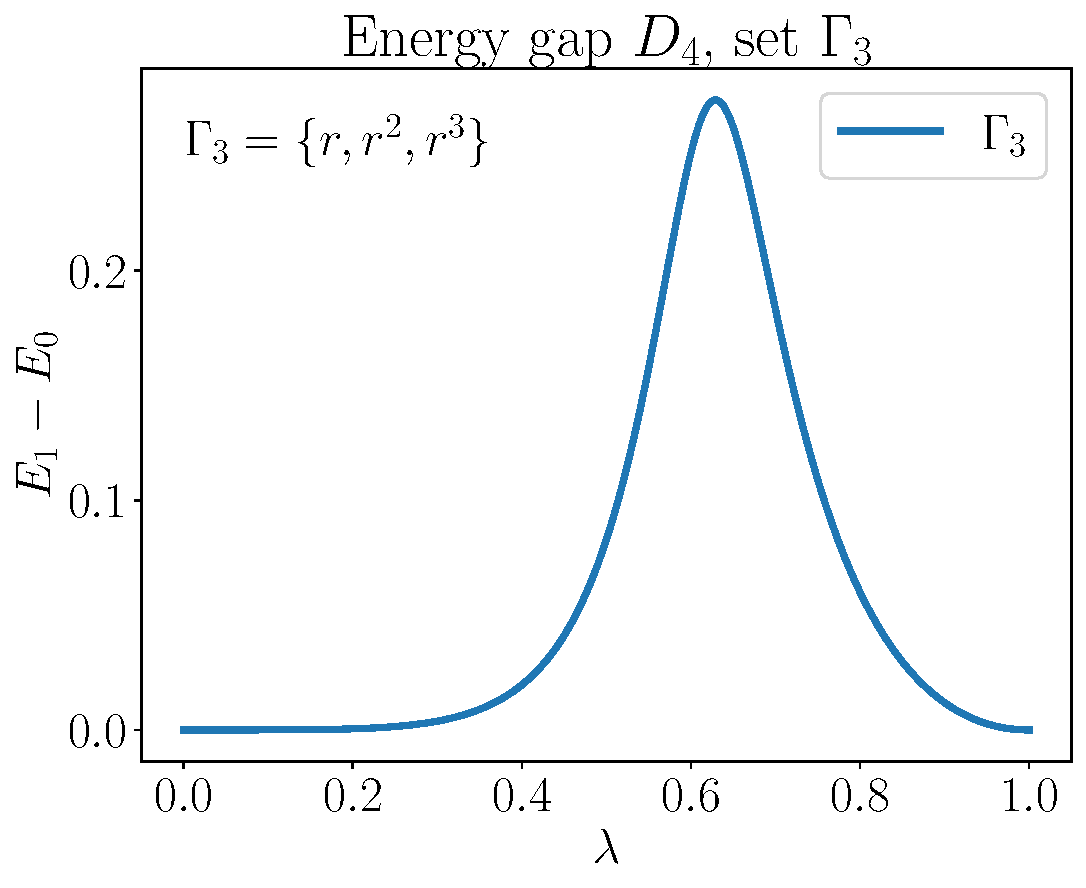
\includegraphics[height=5cm]{assets/graphs/energy_gap_D4_3.pdf}%
    \caption[Ground state gap for $D_4$]{
        \emph{Left:} Energy gap $E_1 - E_0$ for $\Gamma_1$ and $\Gamma_2$.
        \emph{Right:} Energy gap $E_1 - E_0$ for only $\Gamma_3$.
        While the behaviour of the ground state energy may seem the same for all the three generating sets (see Fig.~\ref{fig:ground_state_energy_D4}), the same cannot be said for the energy gaps.
        This is motivated from the fact that $\Gamma_3$ does not generate the whole group, so there is a two-fold degeneracy in the electric eigenvalues for each link.
    }%
    \label{fig:energy_gap_D4}
\end{figure}



\clearpage

\vspace*{1cm}

\begin{figure}[h]
    \centering
    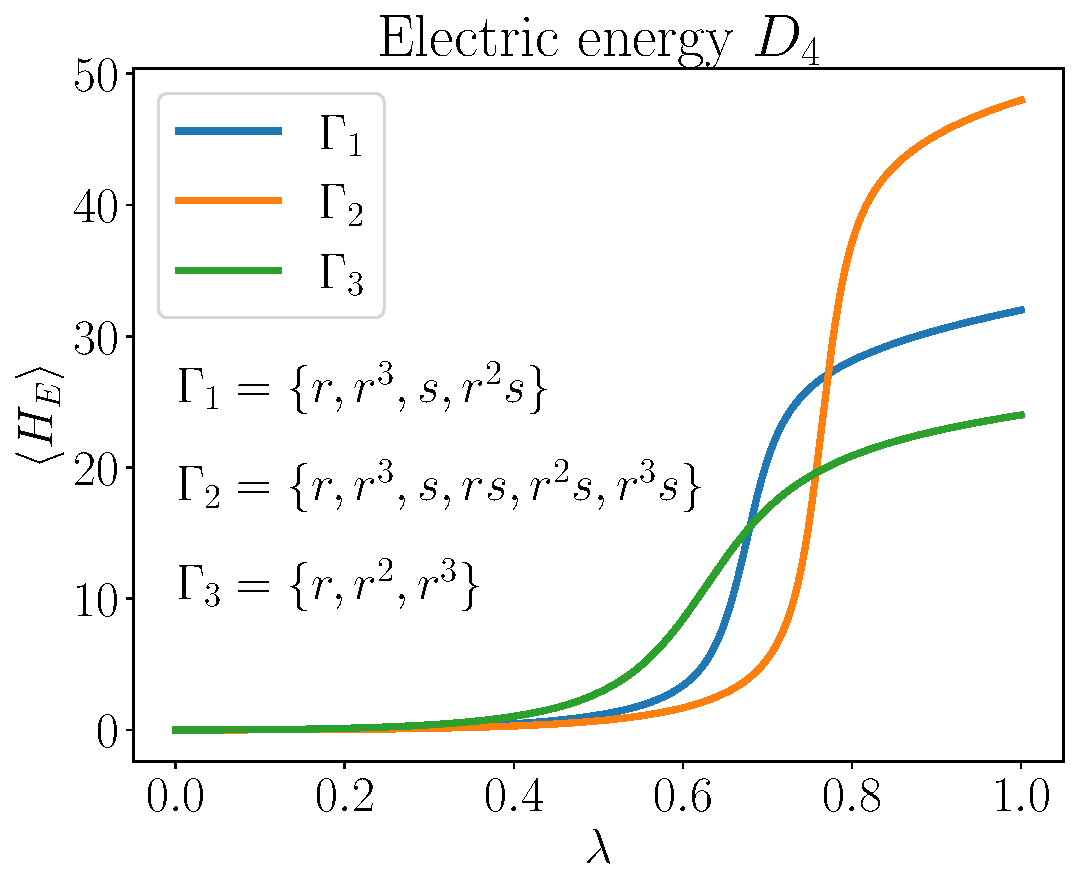
\includegraphics[height=5cm]{assets/graphs/gs_elec_comparison_1_2_3.pdf}%
    \hfill%
    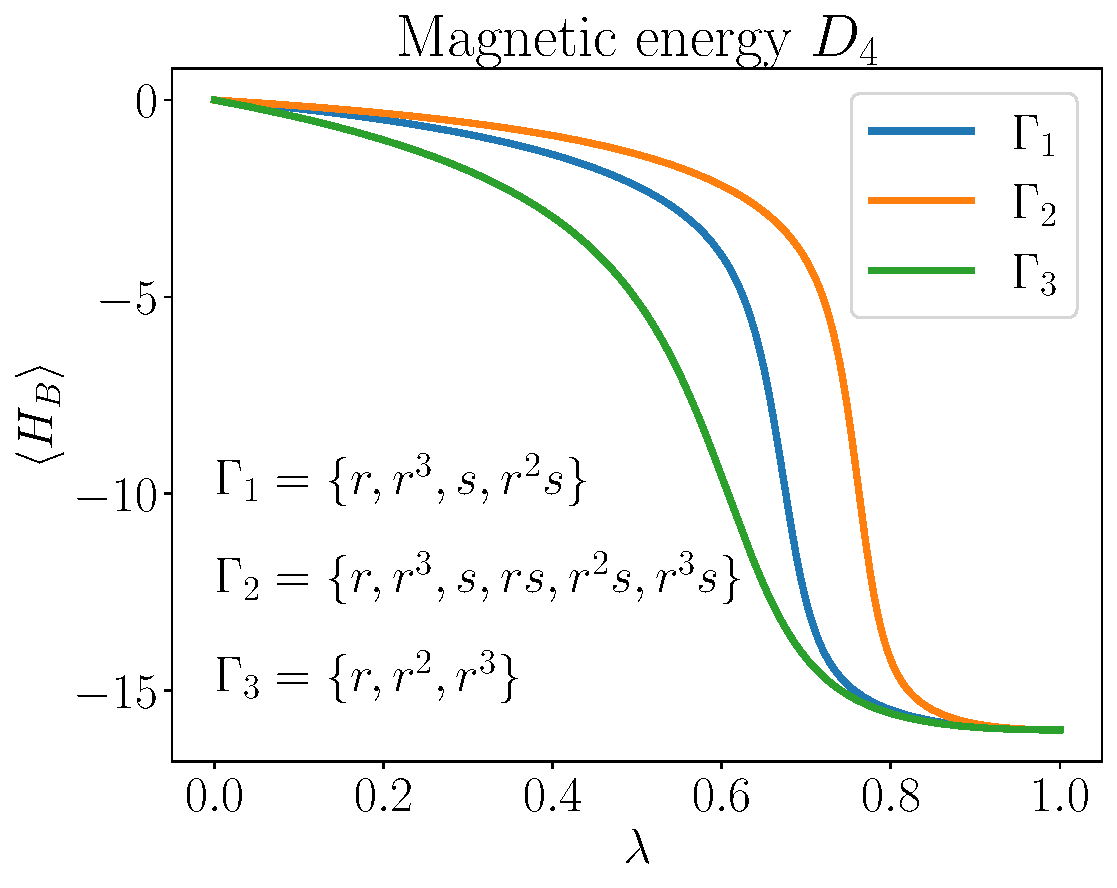
\includegraphics[height=5cm]{assets/graphs/gs_magn_comparison_1_2_3.pdf}
    \caption[Electric and magnetic energies for $D_4$]{%
        Expectation values $\ev*{H_E}$ (\emph{left}) and $\ev*{H_B}$ (\emph{right}).
        They confirm the picture suggested from Fig.~\ref{fig:ground_state_energy_D4}, where there is a transition region for $ 0.6 \lesssim \lambda 0.8 \lesssim 0.8$.
    }
    \label{fig:HE_HB_expt_val_D4}
\end{figure}

\vspace*{0.5cm}

\begin{figure}[h]
    \centering
    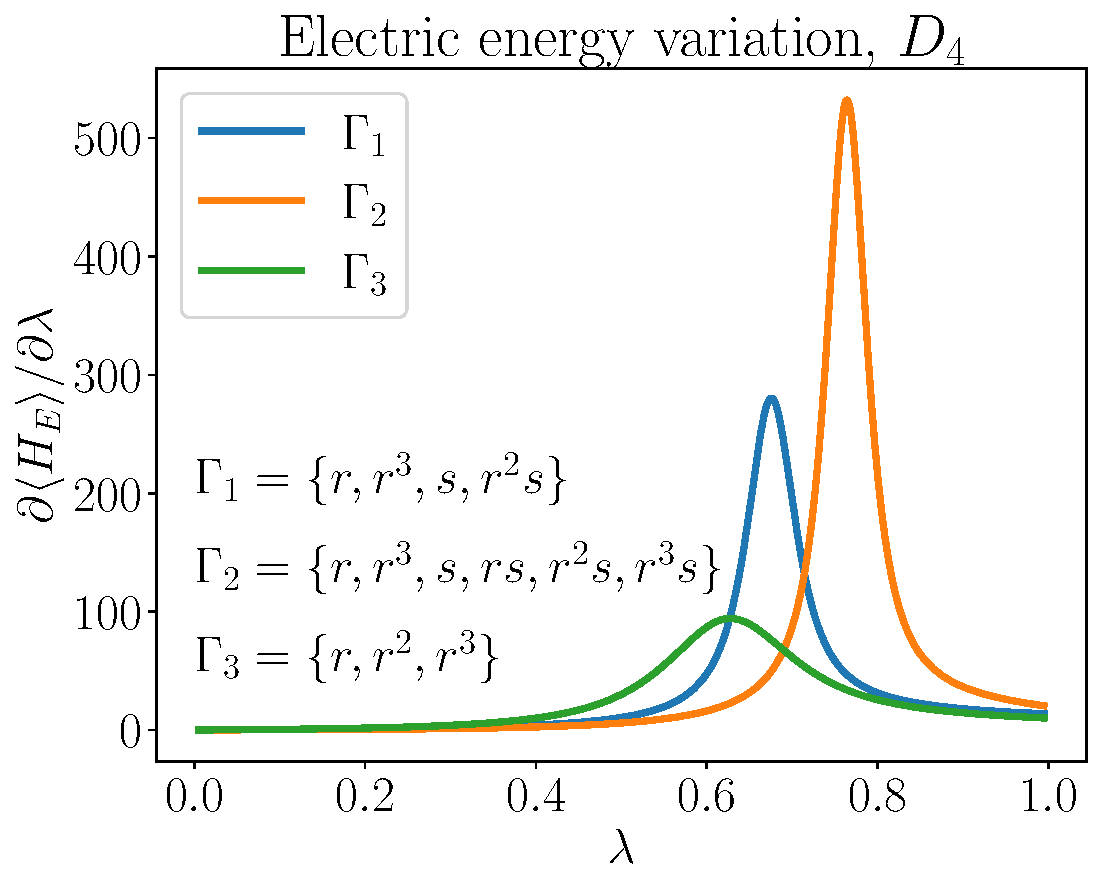
\includegraphics[height=5cm]{assets/graphs/elec_variations_D4.pdf}%
    \hfill%
    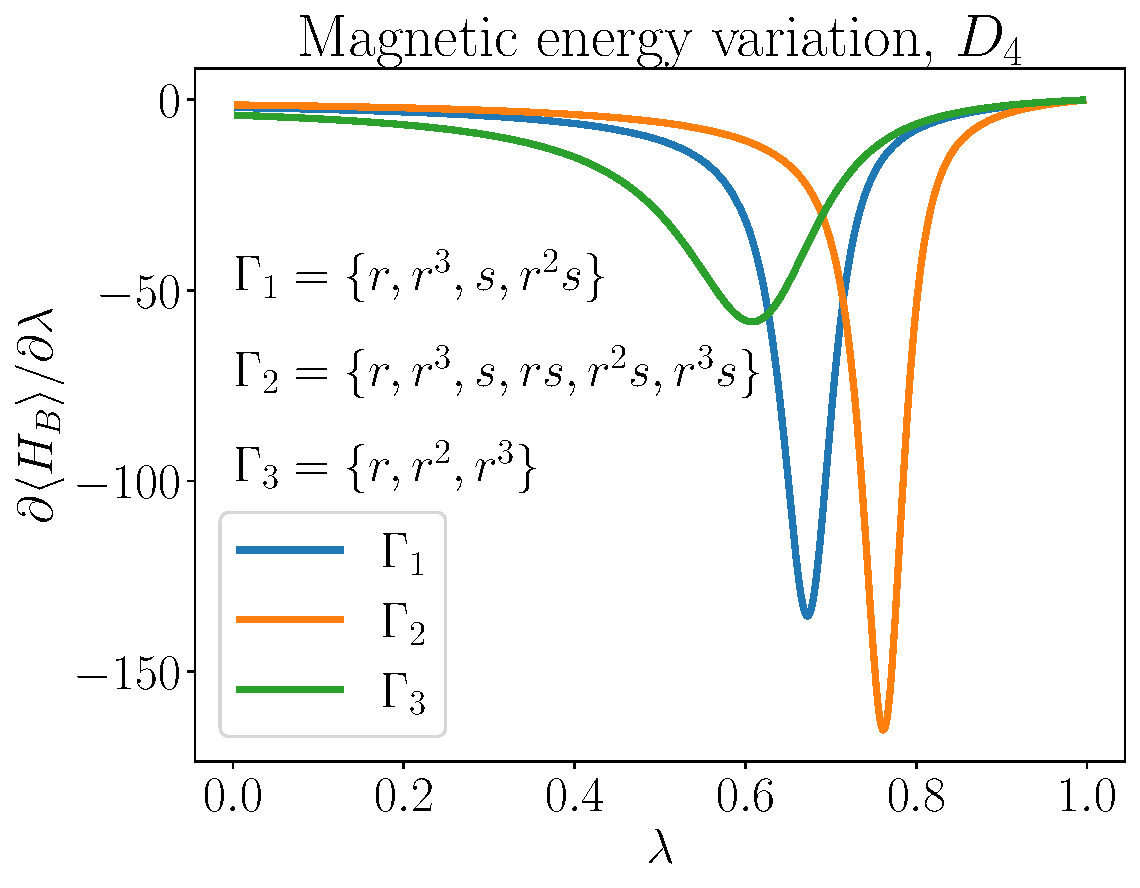
\includegraphics[height=5cm]{assets/graphs/magn_variations_D4.pdf}
    \caption[Electric and magnetic energy variations for $D_4$]{%
        Variations of the expectation values $\ev*{H_E}$ (\emph{left}) and $\ev*{H_B}$ (\emph{right}).
        The location of the peaks can be used identifying the transition points.
        They coincide for $\Gamma_1$ ($\lambda^{\ast} = 0.67(1$) and $\Gamma_2$ ($\lambda^{\ast} = 0.76(1)$) and slightly differs for $\Gamma_3$ ($\lambda_E^{\ast} = 0.63(1)$ and $\lambda_B^{\ast} = 0.61(1)$).
        It should be noted that for $\Gamma_3$ the peak is much smoother, so the identification of the transition point is much more difficult.
    }
    \label{fig:HE_HB_variation_D4}
\end{figure}



\clearpage

\begin{figure}[t]
    \centering
    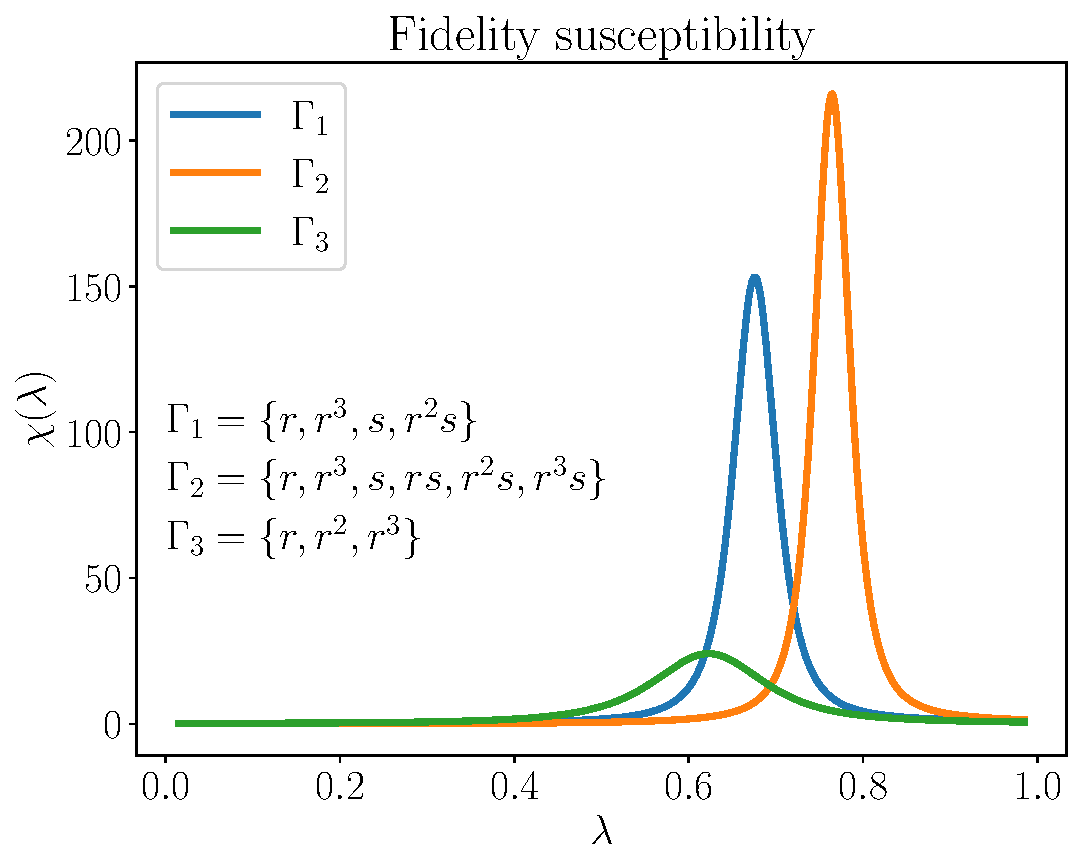
\includegraphics[width=8cm]{assets/graphs/fidelity_susc.pdf}
    \caption[Fidelity susceptibility for $D_4$]{%
        Fidelity susceptibility $\chi(\lambda)$ for $D_4$ for all the three sets $\Gamma_1$, $\Gamma_2$ and $\Gamma_3$.
        The peaks of $\chi(\lambda)$ identifies the transition points for each case.
        The position of such peaks are compatible with those in Fig.~\ref{fig:HE_HB_variation_D4}.
        We find $\lambda_{1, \chi}^*=0.67(1)$, $\lambda_{2, \chi}^*=0.76(1)$ and $\lambda_{3, \chi}^*=0.62(1)$ for $\Gamma_1$, $\Gamma_2$ and $\Gamma_3$, respectively.
    }
    \label{fig:fidelity_D4}
\end{figure}

